\documentclass[sigconf]{acmart}
\usepackage{pgfplots}
\usepackage{colortbl}
\pgfplotsset{width=7cm,compat=1.8}

%%
%% \BibTeX command to typeset BibTeX logo in the docs
\AtBeginDocument{%
  \providecommand\BibTeX{{%
    Bib\TeX}}}

%% Rights management information.  This information is sent to you
%% when you complete the rights form.  These commands have SAMPLE
%% values in them; it is your responsibility as an author to replace
%% the commands and values with those provided to you when you
%% complete the rights form.
\setcopyright{none}
% \setcopyright{acmlicensed}
% \copyrightyear{2018}
% \acmYear{2018}
% \acmDOI{XXXXXXX.XXXXXXX}

%% These commands are for a PROCEEDINGS abstract or paper.
% \acmConference[Conference acronym 'XX]{Make sure to enter the correct
  % conference title from your rights confirmation emai}{June 03--05,
  % 2018}{Woodstock, NY}
%%
%%  Uncomment \acmBooktitle if the title of the proceedings is different
%%  from ``Proceedings of ...''!
%%
%%\acmBooktitle{Woodstock '18: ACM Symposium on Neural Gaze Detection,
%%  June 03--05, 2018, Woodstock, NY}
% \acmISBN{978-1-4503-XXXX-X/18/06}

%%
%% Submission ID.
%%\acmSubmissionID{123-A56-BU3}

%%
%% end of the preamble, start of the body of the document source.
\begin{document}

%%
%% The "title" command has an optional parameter,
%% allowing the author to define a "short title" to be used in page headers.
\title[Unlock the FoundationDB Record Layer]{Unlock the FoundationDB Record Layer: Language Flexibility and Network Freedom with a gRPC Microservice}

%%
%% The "author" command and its associated commands are used to define
%% the authors and their affiliations.
%% Of note is the shared affiliation of the first two authors, and the
%% "authornote" and "authornotemark" commands
%% used to denote shared contribution to the research.
\author{James Krepelka}
\email{jkrepelka@csuchico.edu}
\affiliation{%
  \institution{California State University, Chico}
  \city{Chico}
  \state{California}
  \country{USA}
}

\begin{abstract}
    This paper examines the FoundationDB Record Layer, a Java library enabling record-oriented data storage within the scalable NewSQL FoundationDB database. While powerful, the Record Layer's Java-only implementation and network co-location requirement limit its broader adoption. This research explores the feasibility of encapsulating the Record Layer within a gRPC microservice to address these limitations.
    
    A gRPC microservice layer was implemented, and its performance impact was evaluated against direct Record Layer usage. Experimental results demonstrate that while some overhead is introduced, particularly for read operations, the gRPC approach significantly expands language accessibility and architectural flexibility. For write-heavy workloads, the performance overhead is minimal (1-6\%). This makes the gRPC-enabled Record Layer a compelling option for developers seeking FoundationDB's scalability and ACID guarantees without language or network constraints.
    
    Future work directions include optimizing protobuf handling within the microservice and exploring the development of a "Relationship Layer" to support richer relational data modeling on top of the Record Layer.
\end{abstract}

\begin{CCSXML}
<ccs2012>
   <concept>
       <concept_id>10002951.10002952.10003400.10003401</concept_id>
       <concept_desc>Information systems~Database web servers</concept_desc>
       <concept_significance>500</concept_significance>
       </concept>
   <concept>
       <concept_id>10002951.10002952.10003190.10003195.10010836</concept_id>
       <concept_desc>Information systems~Key-value stores</concept_desc>
       <concept_significance>300</concept_significance>
       </concept>
 </ccs2012>
\end{CCSXML}

\ccsdesc[500]{Information systems~Database web servers}
\ccsdesc[300]{Information systems~Key-value stores}

%%
%% Keywords. The author(s) should pick words that accurately describe
%% the work being presented. Separate the keywords with commas.
\keywords{FoundationDB, distributed databases, gRPC}

%%
%% This command processes the author and affiliation and title
%% information and builds the first part of the formatted document.
\maketitle

\section{Introduction}
\subsection{Database Evolution and the Rise of NewSQL}
Relational databases built upon SQL have dominated data storage since the 1970s \cite{CoddTheory}. However, the scalability demands of Web 2.0 applications exposed limitations in traditional SQL systems. This led to the emergence of NoSQL databases that prioritized scalability and availability, often at the cost of strict consistency guarantees \cite{NewSQL}. While offering advantages, the lack of ACID transactions in many NoSQL systems created complexity for developers accustomed to the transactional guarantees of SQL \cite{NewSQL}.

NewSQL technologies, such as FoundationDB, emerged to bridge this gap. They seek to provide scalable, distributed data storage while maintaining ACID compliance. FoundationDB takes this concept further by proposing a fundamental separation of data models, query languages, and storage engines\cite{FoundationDBPaper}. This approach emphasizes the key-value store as a basic building block, with higher-order data models and query capabilities implemented as composable "Layers."

\subsection{FoundationDB's Record Layer}
FoundationDB's Record Layer (2018) is a notable example of this layered approach. It provides a record-oriented storage model akin to relational databases, featuring structured types, indexes, and basic querying capabilities. This layer is of particular interest because it illustrates both the possibilities and potential limitations of FoundationDB's design philosophy.

The Record Layer is primarily vended as a Java library and interacts with each node in the FoundationDB cluster as needed. This means that the primary use case supported by the Record Layer is to be imported and used by a Java application that runs in the same network as the FoundationDB cluster itself.

\subsection{Research Focus and Thesis}
This paper examines the FoundationDB Record Layer in the context of contemporary database trends. I suggest that the Record Layer's Java-only implementation limits its potential impact and broader adoption, and the network co-location requirement hinders modern deployment practices and security models. Exposing the FoundationDB Record Layer through a microservice would significantly expand its accessibility and compatibility with modern development practices, so long as it doesn't compromise the performance of interactions with FoundationDB.

\section{Literature Review}

\subsection{SQL and the Origins of Relational Databases}

Modern databases have their roots in Dr. E.F. Codd's 1970 proposal of the relational model \cite{CoddTheory}  led to the introduction of Structured English Query Language (SEQUEL, later shortened to SQL) \cite{SEQUEL}. SQL technologies dominated the data storage landscape until the rise of Web 2.0 and its unprecedented scaling demands.

\subsection{The Rise of NoSQL and the CAP Theorem}

Web 2.0 companies faced limitations when trying to scale traditional SQL databases. This led to the emergence of NoSQL technologies in the mid-2000s, such as Google's Bigtable (2005)\cite{BigTable}, Amazon Dynamo (2007)\cite{Dynamo}, and Facebook's Cassandra (2009)\cite{Cassandra}. These solutions were designed for high scalability in the face of massive data growth.

However, Eric Brewer, in his 2000 keynote, presented the CAP theorem \cite{Brewer,Browne_2009}. This theorem posits that distributed systems can only guarantee two out of three properties: Consistency, Availability, and Partition tolerance \cite{BrewerSupport}. NoSQL's emphasis on availability and partition tolerance often came at the expense of consistency, creating challenges for developers in ensuring data integrity.

\subsection{ACID and the Emergence of NewSQL}

The lack of ACID (Atomicity, Consistency, Isolation, Durability) compliance in NoSQL systems became a barrier for many developers \cite{NewSQL}. NewSQL technologies emerged in the early 2010s, aiming to bridge the gap by offering ACID compliance alongside horizontal scalability \cite{NewSQL}. FoundationDB, released in 2010 \cite{FoundationDBCreation}, gained prominence for its highly scalable, fault-tolerant design and flexible data models \cite{FoundationDBPaper,Snowflake}. FoundationDB's emphasis on ACID transactions enabled developers to regain the transactional guarantees familiar from traditional SQL systems.

\subsection{FoundationDB's Innovations and Differentiators}

FoundationDB stands out with its core design philosophy of separating the data model, query language, and storage engine \cite{FoundationDBPaper}. This allows developers to build custom "Layers" to store and access data in diverse formats, including tables, documents, and graphs. FoundationDB's Record and Document Layers demonstrate this flexibility. The Record Layer provides features familiar to SQL users, while the Document Layer acts as a drop-in replacement for MongoDB, easing migration \cite{FDBDocumentGithub}.

\subsection{FoundationDB's Shortcomings and Potential}

Despite its advantages, FoundationDB faces limitations that may hinder its wider adoption. The Record Layer's restriction to Java and its requirement to be on the same network as the cluster are potential barriers. Addressing these limitations could significantly expand FoundationDB's reach.

\section{Evaluation Environment Setup}

\begin{figure}[t]
  \centering
  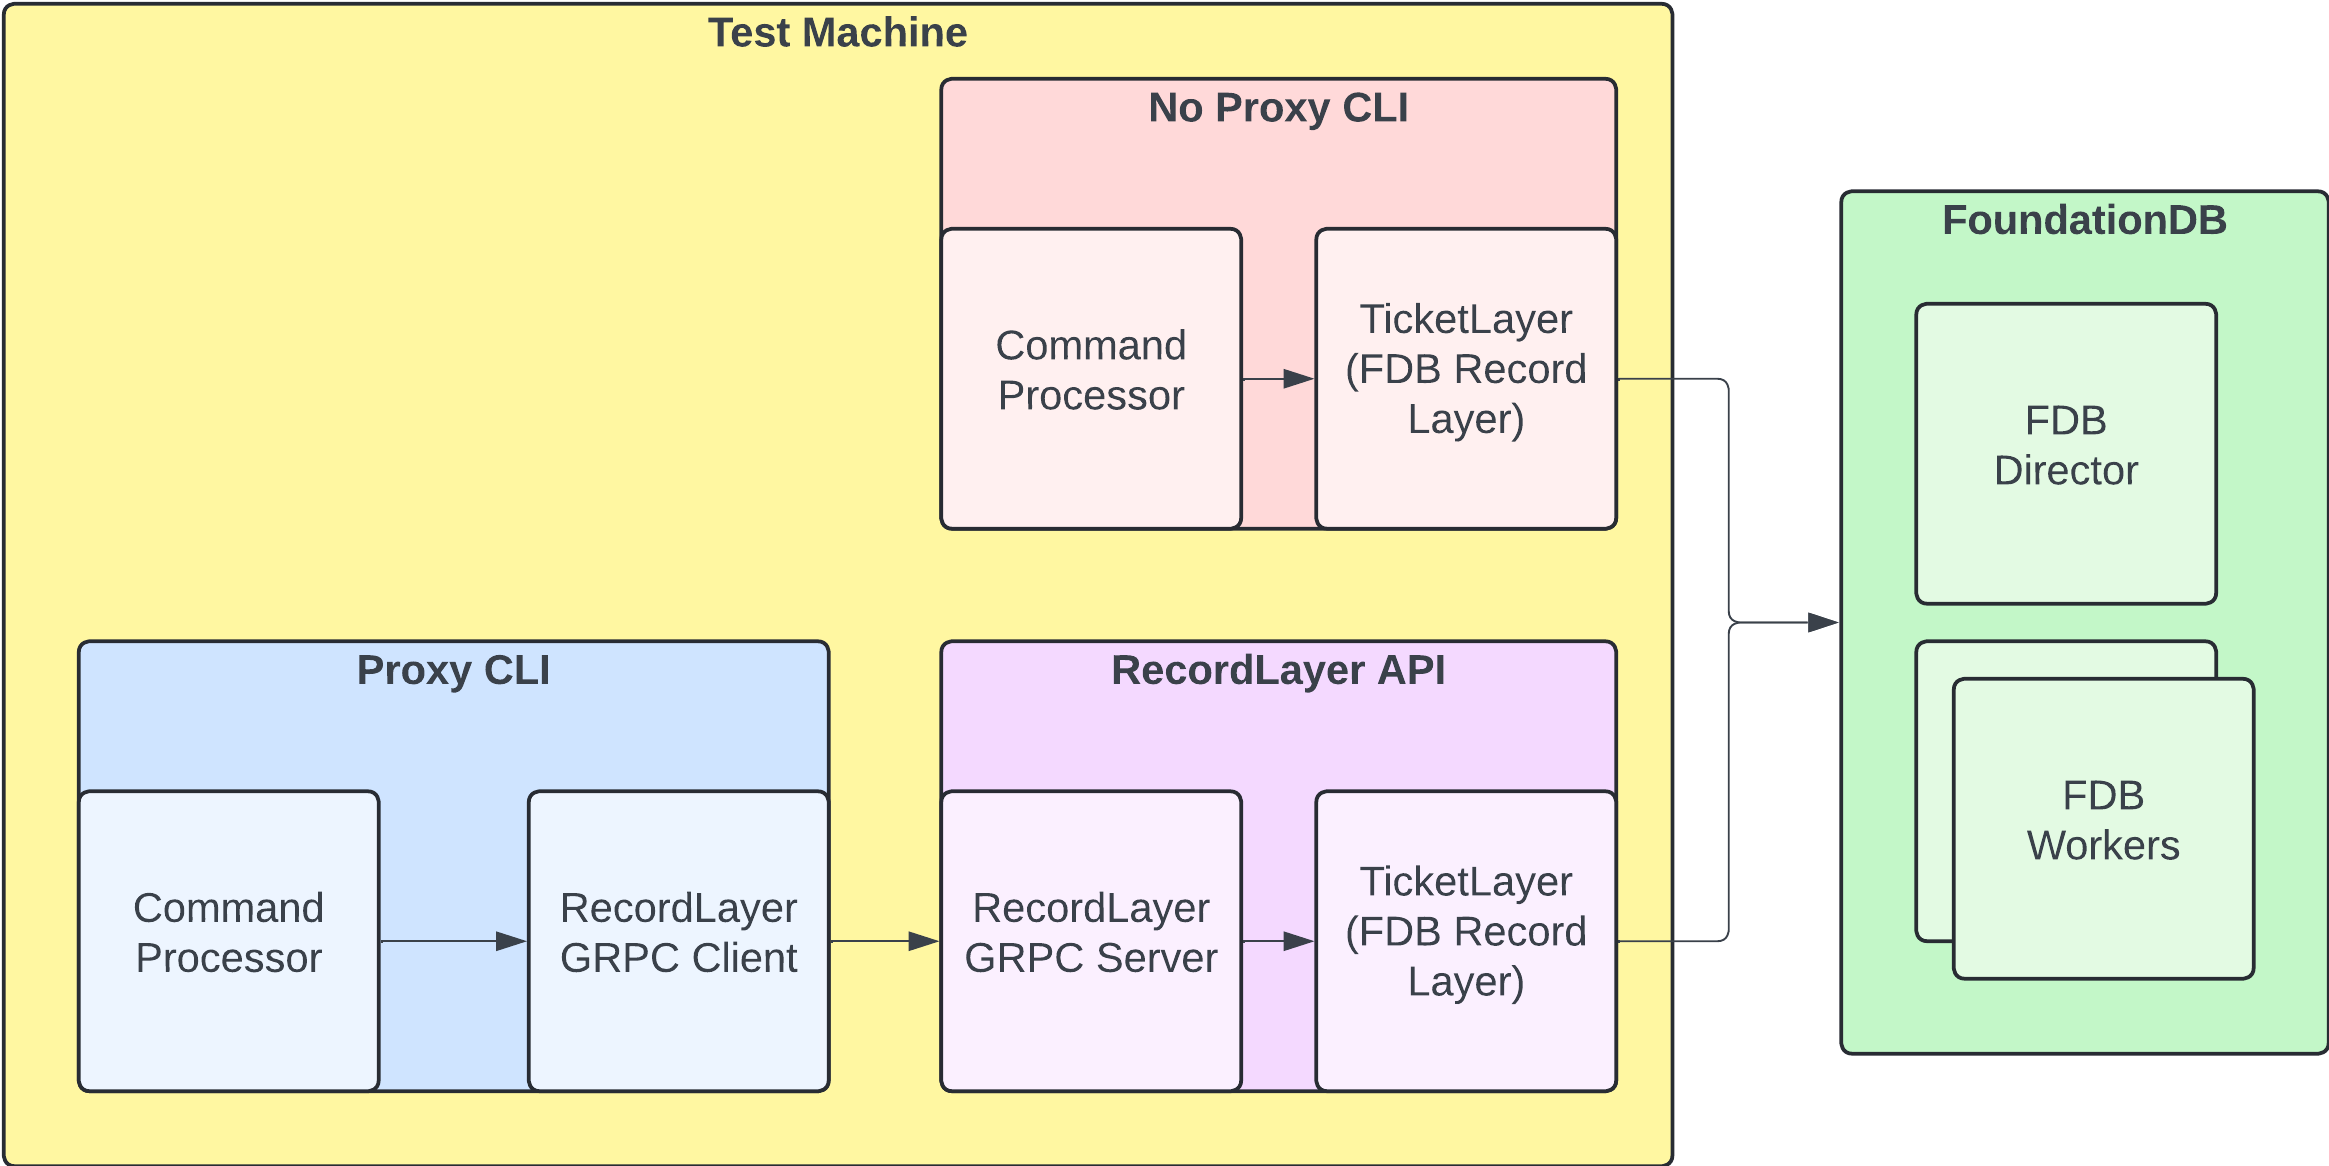
\includegraphics[width=\linewidth]{diag_system.png}
  \caption{An overview of the system architecture for the experiment.}
  \Description{A yellow square labeled test machine contains squares for No Proxy CLI, Proxy CLI and RecordLayer API. Next to the yellow square is a green square labeled FoundationDB.}
  \label{fig:diag_system}
\end{figure}

This section provides a comprehensive overview of all the components of the experiment (Figure \ref{fig:diag_system}). I will describe the process of writing the code for the experiment and the configuration of the testing environment in detail.

\subsection{Code}

To evaluate the time added by a gRPC API built around the Record Layer, I built a common TicketLayer library that the two different CLIs use.

\subsubsection{TicketLayer Library}

I implemented a shared TicketLayer library as a Data Access Layer (DAL). This DAL provides consistent save and get operations for interacting with the FoundationDB Record Layer. Employing this shared DAL across both the CLI and server components guarantees experimental consistency.

\subsubsection{No Proxy CLI}

\begin{figure}[h]
  \centering
  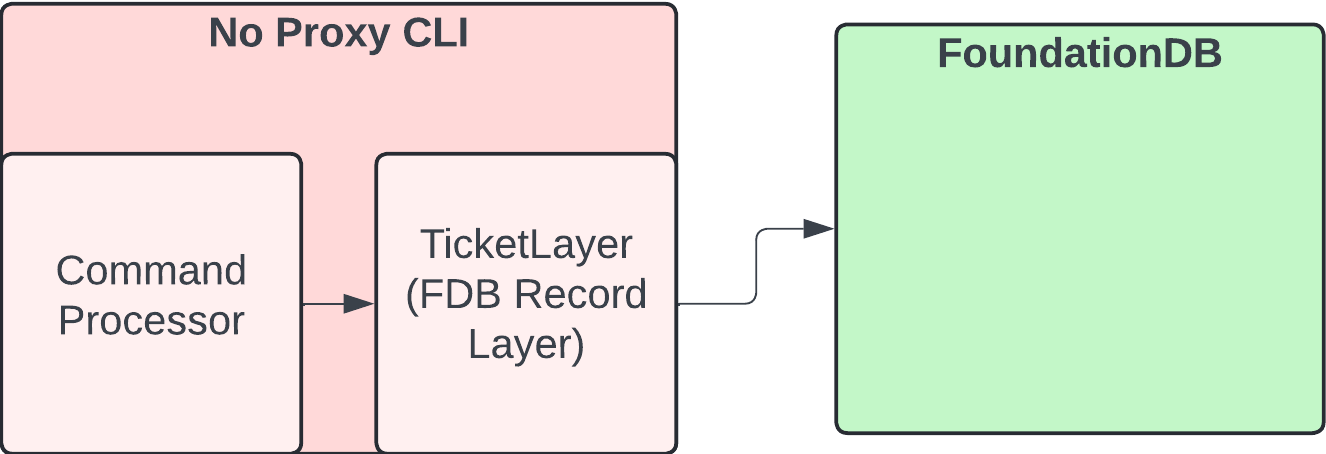
\includegraphics[width=\linewidth]{diag_code_npc.png}
  \caption{An overview of how the No Proxy CLI directly interacts with FoundationDB.}
  \Description{A red square containing two light red squares. The first light red square contains the text Command Processor and points to the second light red square that contains TicketLayer. The second light red square points to a green square outside of the red square. The green square contains the word FoundationDB.}
  \label{fig:diag_code_npc}
\end{figure}

The No Proxy Command-Line Interface (CLI) is implemented in the Java programming language. It leverages the Record Layer as a third-party library and establishes network connections directly with FoundationDB nodes. The CLI comprises two distinct components: a command processor that accepts user commands for interacting with FoundationDB, and the TicketLayer library, which utilizes the FoundationDB Record Layer library to facilitate connectivity (Figure \ref{fig:diag_code_npc}).

\subsubsection{Proxy CLI}

\begin{figure}[h]
  \centering
  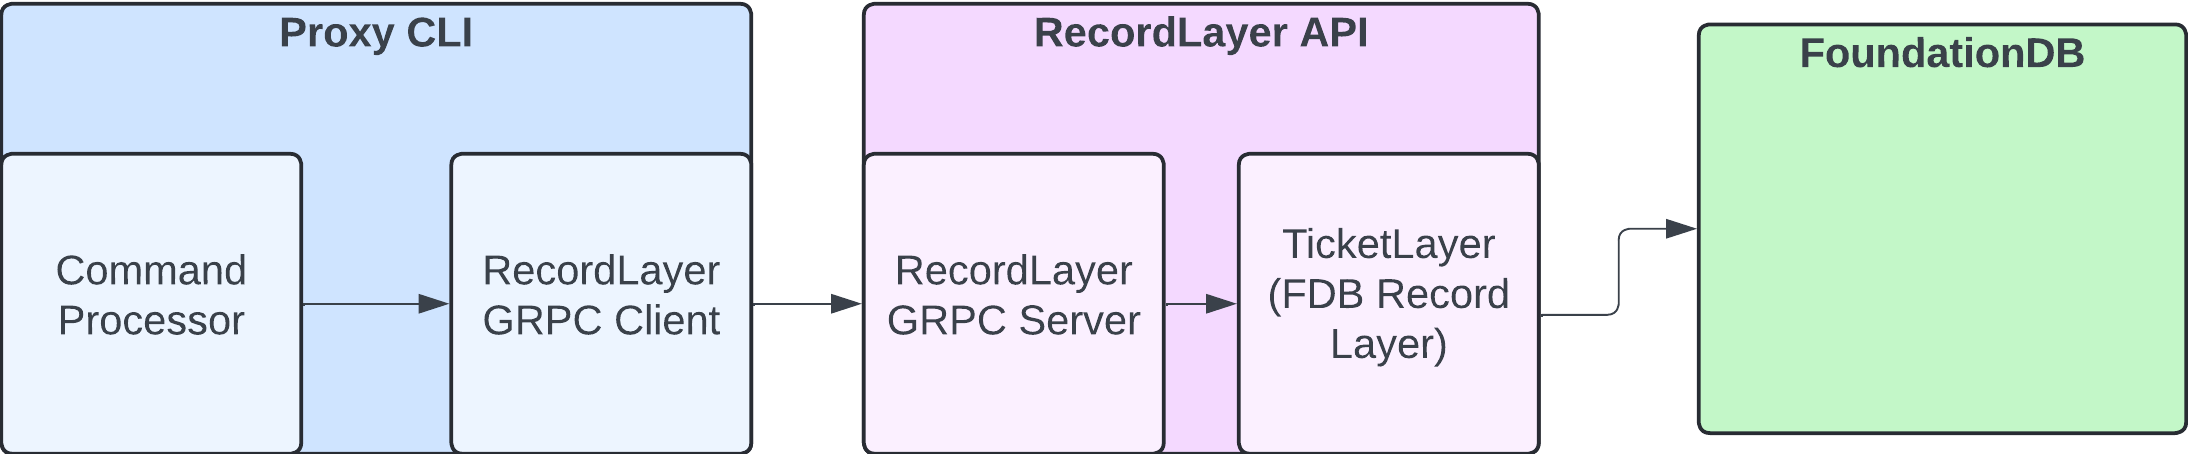
\includegraphics[width=\linewidth]{diag_code_pc.png}
  \caption{An overview of how the Proxy CLI interacts with the RecordLayer API, which then interacts with FoundationDB.}
  \Description{A blue square containing two light blue squares. The first light blue square contains the text Command Processor and points to the second light blue square that contains gRPC Client. The second light blue square points to a purple square that contains two light purple squares. The first light purple square contains the text gRPC Server and points to the second light purple square that contains TicketLayer. The second light purple square points to a green square outside of the purple square. The green square contains the word FoundationDB.}
  \label{fig:diag_code_pc}
\end{figure}

The Proxy CLI approach involves two Java binaries: the Proxy CLI and the RecordLayer API server (Figure \ref{fig:diag_code_pc}).

This Java implementation maintains consistency with the No Proxy CLI for comparative testing.
Importantly, the Proxy CLI could be written in any language supported by gRPC (currently 11, see https://grpc.io/docs/languages/).

The Proxy CLI includes a command processor, mirroring the No Proxy CLI for consistent user interaction, and a generated gRPC client library. The RecordLayer API server comprises a generated gRPC server and the shared TicketLayer library for FoundationDB access.

This scenario evaluates the performance overhead introduced by the gRPC layer in facilitating FoundationDB interactions.

\subsection{Hardware Configuration}

\begin{figure}[h]
  \centering
  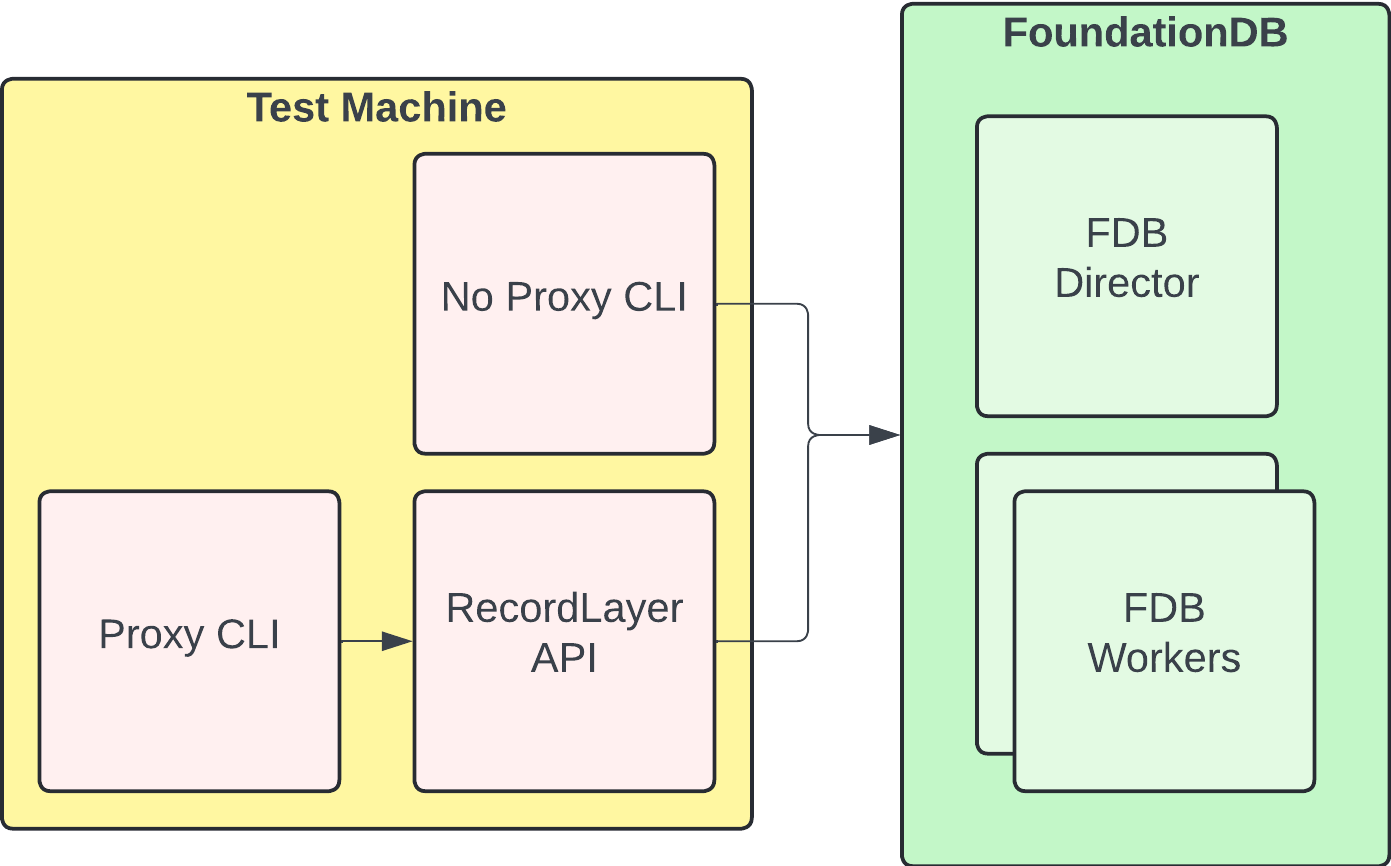
\includegraphics[width=\linewidth]{diag_machines.png}
  \caption{An overview of the machine configuration and locations where the CLIs were executed.}
  \Description{A yellow square labeled Test Machine contains 3 red squares. One red square containing No Proxy CLI points out to the green FoundationDB box sitting next to the yellow square. Another red square containing Proxy CLI points at a red box containing RecordLayer API, which points at the same green FoundationDB square.}
  \label{fig:diag_machines}
\end{figure}

For the purpose of acquiring timing-related data for this experiment, four individual machines were utilized (Figure \ref{fig:diag_machines}), all of which were operational within the confines of a singular server rack.

Since the focus is on the overhead of the gRPC layer, detailed hardware specifications of the FoundationDB cluster are less critical. However, providing a high-level overview ensures reproducibility.

\subsubsection{Test Machine}

\begin{itemize}
\item {\texttt{OS}}: Linux 6.8.2
\item{\texttt{RAM}}: 256 GiB (3200MHz DDR4)
\item{\texttt{Storage}}: 20+ TB NVMe (ZFS)
\item{\texttt{Network}}: 1GB link to FoundationDB cluster (same rack)
\end{itemize}

\subsubsection{FoundationDB Cluster (3 nodes)}

\begin{itemize}
    \item {\texttt{foundationdb.conf}}: paper/supporting/foundationdb.conf
    \item {\texttt{OS}}: Linux 6.8.2
    \item{\texttt{RAM}}: 128 GiB per node (3200MHz+, one at 4800MHz)
    \item{\texttt{Storage}}: 20+ TB NVMe (ZFS)
    \begin{itemize}
        \item{\texttt{Log}}: 54GiB Intel® Optane™ P1600X
        \item{\texttt{Data}}: 2TB Crucial MX500 or 2TB 870 EVO SATA SSDs
    \end{itemize}
    \item{\texttt{Network}}: 10GB interconnects
\end{itemize}

\section{Evaluation Data}

\subsection{Experimental Methodology}

Four performance tests were conducted, each comparing the Proxy CLI and No Proxy CLI setups described in Section 2. Both CLIs executed the same commands with incrementally increasing arguments. To ensure accurate timing, a timing mechanism was implemented around each command. This process was repeated 20 times per CLI and argument combination. Data points in subsequent charts represent the average runtime across these 20 executions, with a measured confidence level exceeding 99.9%.

\subsection{Single Read Evaluation}

To assess single record retrieval, the \textbf{get-single N} command was executed on both Proxy and No Proxy CLIs with increasing values of \textbf{N} (1,000 to 40,000). The test dataset consisted of 75,000 randomly generated 'Ticket' objects stored in FoundationDB. Prior to timed runs, 1,000 test objects were randomly selected from the dataset. Performance measurements were taken as each CLI retrieved these 1,000 objects individually.

\subsubsection{Data}

Below is the collected data in bar-chart and tabular formats.

\begin{figure}[h]
    \centering
    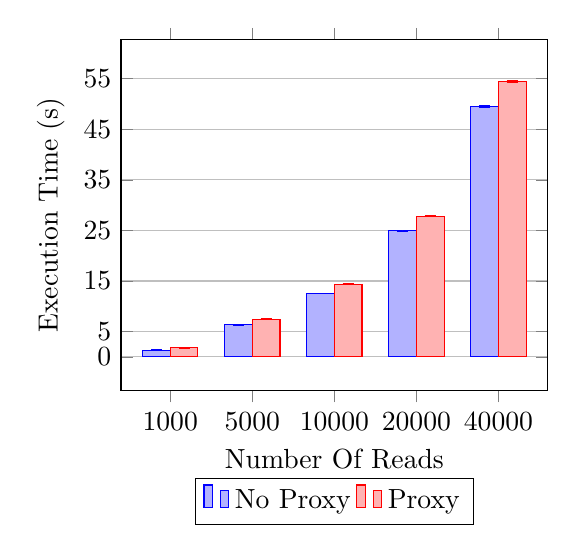
\begin{tikzpicture}
        \begin{axis}[
            ybar = 0pt,
            enlargelimits=0.15,
            legend style={at={(0.5,-0.25)},
            anchor=north,legend columns=-1},
            ylabel={Execution Time (s)},
            xlabel={Number Of Reads},
            symbolic x coords={1000, 5000, 10000, 20000, 40000},
            ytick={
                0, 5000, 15000, 25000, 35000, 45000, 55000
            },
            yticklabels={
                0, $5$, $15$, $25$, $35$, $45$, $55$
            },
            ymajorgrids=true,
            xtick=data,
            scaled ticks = false
        ]
            \addplot+[
                error bars/.cd,
                y dir=both,
                y explicit
            ] coordinates {
                (1000, 1335.4) +- (0.0, 15.5)
                (5000, 6319.5) +- (0.0, 60.4)
                (10000, 12525.05) +- (0.0, 81.5)
                (20000, 24936.7) +- (0.0, 120)
                (40000, 49522.8) +- (0.0, 199.9)
            };
        
            \addplot+[
                error bars/.cd,
                y dir=both,
                y explicit
            ] coordinates {
                (1000, 1782.35) +- (0.0, 80.9)
                (5000, 7447.65) +- (0.0, 72)
                (10000, 14354.1) +- (0.0, 87)
                (20000, 27815) +- (0.0, 143)
                (40000, 54526) +- (0.0, 173.5)
            };
            
            \legend{No Proxy, Proxy}
        \end{axis}
    \end{tikzpicture}
    \caption{The number of reads plotted against the time it took to execute them.}
    \Description{A bar chart of data from the single read experiment.}
\end{figure}

\begin{table}[h]
\begin{tabular}{|c|l|l|c|}
    \hline
    \rowcolor[HTML]{656565} 
    \multicolumn{1}{|c}{\cellcolor[HTML]{656565}{\color[HTML]{FFFFFF} \textbf{N}}} &
    {\color[HTML]{FFFFFF} \textbf{NoProxy (ms)}} &
    {\color[HTML]{FFFFFF} \textbf{Proxy (ms)}} &
    {\color[HTML]{FFFFFF} \textbf{\% Inc}} \\ \hline
    1,000  & 1,335.40 +/- 15.48   & 1,782.35 +/- 80.91 & 33.47\% \\
    \rowcolor[HTML]{EFEFEF} 
    5,000  & 6,319.50 +/- 60.42   & 7,447.65 +/- 72.04 & 17.85\% \\
    10,000 & 12,525.05 +/- 81.47 & 14,354.10 +/- 87.04 & 14.60\% \\
    \rowcolor[HTML]{EFEFEF} 
    20,000 & 24,936.70 +/- 119.98 & 27,815.0 +/- 143.04  & 11.54\% \\
    40,000 & 49,522.80 +/- 199.89 & 54,526.0 +/- 173.46  & 10.10\% \\ \hline
\end{tabular}
\caption{The number of reads, how long they took to execute in milliseconds, +/- the measured error, and the percentage increase in runtime of the Proxy CLI versus the NoProxy CLI.}
\end{table}

\subsubsection{Partial Conclusion}

The data demonstrates that a gRPC API layer built upon the Record Layer introduces considerable overhead when retrieving single records from the database. In scenarios with a low volume of reads, both runtime increases (33\%) and greater variability (~80ms vs ~15ms) were observed compared to direct Record Layer access. While the overhead decreases with larger numbers of reads (10\%), it remains noticeable.

This finding suggests that for applications requiring high Queries Per Second (QPS) on small-object reads, the performance trade-offs of a gRPC layer warrant careful consideration against the architectural and developer-facing benefits outlined earlier in the paper.

\subsection{Batch Read Evaluation}

To evaluate batch read performance, the \textbf{get-multiple N} command was executed on both Proxy and No Proxy CLIs with increasing values of \textbf{N} (10 to 400). The test involved retrieving the entire dataset of 75,000 randomly generated 'Ticket' objects from FoundationDB. Each retrieval operation was repeated \textbf{N} times within a timed execution.

\subsubsection{Data}

Below is the collected data in bar-chart and tabular formats.

\begin{figure}[h]
    \centering
    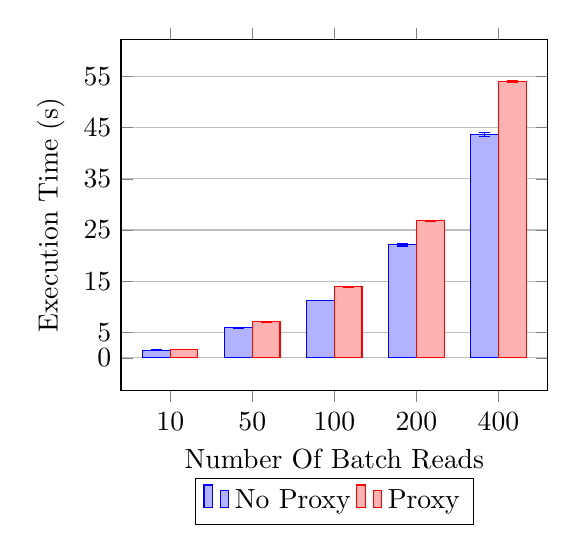
\begin{tikzpicture}
        \begin{axis}[
            ybar = 0pt,
            enlargelimits=0.15,
            legend style={at={(0.5,-0.25)},
            anchor=north,legend columns=-1},
            ylabel={Execution Time (s)},
            xlabel={Number Of Batch Reads},
            symbolic x coords={10,50,100,200,400},
            ytick={
                0, 5000, 15000, 25000, 35000, 45000, 55000
            },
            yticklabels={
                0, $5$, $15$, $25$, $35$, $45$, $55$
            },
            ymajorgrids=true,
            xtick=data,
            scaled ticks = false
        ]
            \addplot+[
                error bars/.cd,
                y dir=both,
                y explicit
            ] coordinates {
                (10, 1526.35) +- (0.0, 15.8)
                (50, 5855.75) +- (0.0, 66.3)
                (100, 11220.4) +- (0.0, 63)
                (200, 22105.75) +- (0.0, 250.4)
                (400, 43695.85) +- (0.0, 348.2)
            };
        
            \addplot+[
                error bars/.cd,
                y dir=both,
                y explicit
            ] coordinates {
                (10, 1642.05) +- (0.0, 18.5)
                (50, 7023.7) +- (0.0, 51)
                (100, 13883.55) +- (0.0, 55)
                (200, 26766.95) +- (0.0, 142.9)
                (400, 54060.25) +- (0.0, 199.8)
            };
            
            \legend{No Proxy, Proxy}
        \end{axis}
    \end{tikzpicture}
    \caption{The number of batch reads plotted against the time it took to execute them.}
    \Description{A bar chart of data from the batch read experiment.}
\end{figure}

\begin{table}[h]
\begin{tabular}{|c|l|l|c|}
    \hline
    \rowcolor[HTML]{656565} 
    \multicolumn{1}{|c}{\cellcolor[HTML]{656565}{\color[HTML]{FFFFFF} \textbf{N}}} &
    {\color[HTML]{FFFFFF} \textbf{NoProxy (ms)}} &
    {\color[HTML]{FFFFFF} \textbf{Proxy (ms)}} &
    {\color[HTML]{FFFFFF} \textbf{\% Inc}} \\ \hline
    10  & 1,526.35 +/- 15.84   & 1,642.05 +/- 18.47   & 7.58\%  \\
    \rowcolor[HTML]{EFEFEF} 
    50  & 5,855.75 +/- 66.25   & 7,023.70 +/- 51.00   & 19.95\% \\
    100 & 11,220.40 +/- 63.00  & 13,883.55 +/- 54.98  & 23.73\% \\
    \rowcolor[HTML]{EFEFEF} 
    200 & 22,105.75 +/- 250.38 & 26,766.95 +/- 142.92 & 21.09\% \\
    400 & 43,695.85 +/- 348.24 & 54,060.25 +/- 199.79 & 23.72\% \\ \hline
\end{tabular}
\caption{The number of batch reads, how long they took to execute in milliseconds, +/- the measured error, and the percentage increase in runtime of the Proxy CLI versus the NoProxy CLI.}
\end{table}

\subsubsection{Partial Conclusion}

Experimental data indicates that the gRPC API layer introduces a non-negligible overhead for batch reads from the database.
For smaller numbers of repeated batch reads, a runtime increase of 7.58\% was observed compared to direct Record Layer access.
This overhead grows to approximately 20\%, with increased variability, as the number of repeated batch reads scales.

While less pronounced than in single-read scenarios, these results suggest that the architectural benefits of a gRPC layer should be weighed against its performance impact, particularly in applications with frequent, large-scale read operations.

\subsection{Single Write Evaluation}

To assess single-object write performance, \textbf{the create-single N} command was executed on both Proxy and No Proxy CLIs with increasing values of \textbf{N} (1,000 to 40,000).
For each test iteration, \textbf{N} randomly generated 'Ticket' objects were created.
The timer was initiated prior to saving these objects individually to FoundationDB.
To maintain a consistent database state, all created objects were deleted before subsequent test runs.

\subsubsection{Data}

Below is the collected data in bar-chart and tabular formats.

\begin{figure}[h]
    \centering
    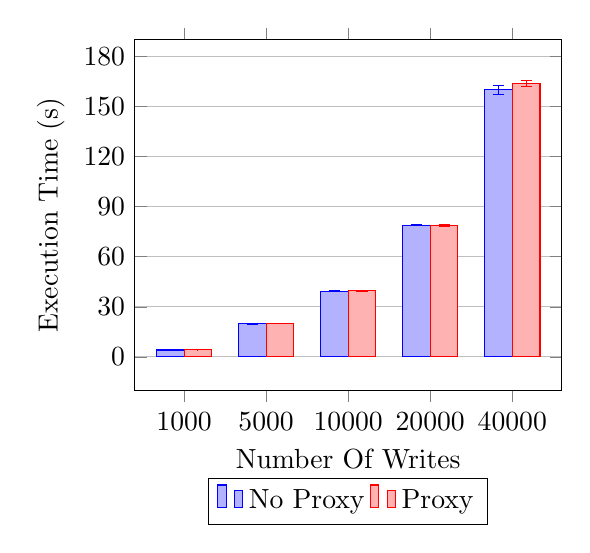
\begin{tikzpicture}
        \begin{axis}[
            ybar = 0pt,
            enlargelimits=0.15,
            legend style={at={(0.5,-0.25)},
            anchor=north,legend columns=-1},
            ylabel={Execution Time (s)},
            xlabel={Number Of Writes},
            symbolic x coords={1000, 5000, 10000, 20000, 40000},
            ytick={
                0, 30000, 60000, 90000, 120000, 150000, 180000
            },
            yticklabels={
                0, $30$, $60$, $90$, $120$, $150$, $180$
            },
            ymajorgrids=true,
            xtick=data,
            scaled ticks = false
        ]
            \addplot+[
                error bars/.cd,
                y dir=both,
                y explicit
            ] coordinates {
                (1000, 4113.5) +- (0.0, 70.7)
                (5000, 19791.8) +- (0.0, 90.9)
                (10000, 39358.35) +- (0.0, 238.3)
                (20000, 78946.55) +- (0.0, 420.6)
                (40000, 159947.95) +- (0.0, 2544.1)
            };
        
            \addplot+[
                error bars/.cd,
                y dir=both,
                y explicit
            ] coordinates {
                (1000, 4305.95) +- (0.0, 49.3)
                (5000, 20045.7) +- (0.0, 126.2)
                (10000, 39577.4) +- (0.0, 185.8)
                (20000, 78803.85) +- (0.0, 434)
                (40000, 163947.5) +- (0.0, 1787.4)
            };
            
            \legend{No Proxy, Proxy}
        \end{axis}
    \end{tikzpicture}
    \caption{The number of writes plotted against the time it took to execute them.}
    \Description{A bar chart of data from the single write experiment.}
\end{figure}

\begin{table}[h]
\begin{tabular}{|c|l|l|c|}
    \hline
    \rowcolor[HTML]{656565} 
    \multicolumn{1}{|c}{\cellcolor[HTML]{656565}{\color[HTML]{FFFFFF} \textbf{N}}} &
    {\color[HTML]{FFFFFF} \textbf{NoProxy (ms)}} &
    {\color[HTML]{FFFFFF} \textbf{Proxy (ms)}} &
    {\color[HTML]{FFFFFF} \textbf{\% Inc}} \\ \hline
    1,000  & 4,113.50 +/- 70.66      & 4,305.95 +/- 49.32      & 4.68\%  \\
    \rowcolor[HTML]{EFEFEF} 
    5,000  & 197,91.80 +/- 90.93     & 20,045.70 +/- 126.23    & 1.28\%  \\
    10,000 & 39,358.35 +/- 238.27    & 39,577.40 +/- 185.76    & 0.56\%  \\
    \rowcolor[HTML]{EFEFEF} 
    20,000 & 78,946.55 +/- 420.61    & 78,803.85 +/- 433.98    & -0.18\% \\
    40,000 & 159,947.95 +/- 2,544.05 & 163,947.50 +/- 1,787.43 & 2.50\%  \\ \hline
\end{tabular}
\caption{The number of writes, how long they took to execute in milliseconds, +/- the measured error, and the percentage increase in runtime of the Proxy CLI versus the NoProxy CLI.}
\end{table}

\subsubsection{Partial Conclusion}

The experimental results indicate that a gRPC API layer introduces minimal overhead when writing small records to the database. In tests with a low volume of writes, a slight runtime increase (4.68\%) was observed for the Proxy CLI. However, this difference becomes negligible as the number of writes increases.

These findings suggest that for write-heavy workloads, employing a gRPC proxy layer has limited performance drawbacks. Consider this alongside the architectural and developer-facing benefits discussed earlier when choosing a FoundationDB Record Layer access strategy

\subsection{Batch Write Evaluation}

For the purpose of conducting this experiment, I executed the \textbf{create-multiple 500 N} command for both the Proxy and No Proxy CLIs, gradually increasing the number of tickets from 10 to 400. During this test, each CLI generated \textbf{500} random ticket objects \textbf{N} times, storing them in distinct lists of \textbf{500} tickets each. Subsequently, the CLIs initiated a timer and proceeded to access each list in FoundationDB via \textbf{N} distinct calls.

Upon completion of the test, I proceeded to delete all tickets from FoundationDB to ensure that subsequent creations occurred within a pristine and empty database.

\subsubsection{Data}

Below is the collected data in bar-chart and tabular formats.

\begin{figure}[h]
    \centering
    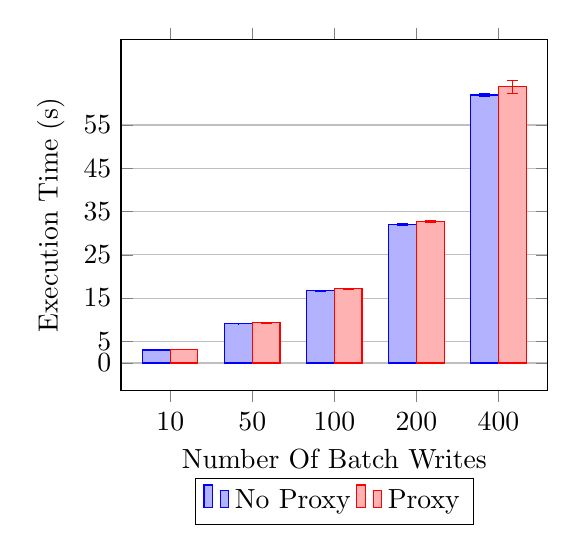
\begin{tikzpicture}
        \begin{axis}[
            ybar = 0pt,
            enlargelimits=0.15,
            legend style={at={(0.5,-0.25)},
            anchor=north,legend columns=-1},
            ylabel={Execution Time (s)},
            xlabel={Number Of Batch Writes},
            symbolic x coords={10,50,100,200,400},
            ytick={
                0, 5000, 15000, 25000, 35000, 45000, 55000
            },
            yticklabels={
                0, $5$, $15$, $25$, $35$, $45$, $55$
            },
            ymajorgrids=true,
            xtick=data,
            scaled ticks = false
        ]
            \addplot+[
                error bars/.cd,
                y dir=both,
                y explicit
            ] coordinates {
                (10, 3005.15) +- (0.0, 42.4)
                (50, 9091.7) +- (0.0, 70.4)
                (100, 16699.3) +- (0.0, 122.7)
                (200, 32001.25) +- (0.0, 132.2)
                (400, 61929.3) +- (0.0, 328)
            };
        
            \addplot+[
                error bars/.cd,
                y dir=both,
                y explicit
            ] coordinates {
                (10, 3185.9) +- (0.0, 29.6)
                (50, 9317.05) +- (0.0, 114.4)
                (100, 17182.35) +- (0.0, 73.6)
                (200, 32699.9) +- (0.0, 248.5)
                (400, 63828.75) +- (0.0, 1523.5)
            };
            
            \legend{No Proxy, Proxy}
        \end{axis}
    \end{tikzpicture}
    \caption{The number of batch writes plotted against the time it took to execute them.}
    \Description{A bar chart of data from the batch write experiment.}
\end{figure}

\begin{table}[h]
\begin{tabular}{|c|l|l|c|}
    \hline
    \rowcolor[HTML]{656565} 
    \multicolumn{1}{|c}{\cellcolor[HTML]{656565}{\color[HTML]{FFFFFF} \textbf{N}}} &
    {\color[HTML]{FFFFFF} \textbf{NoProxy (ms)}} &
    {\color[HTML]{FFFFFF} \textbf{Proxy (ms)}} &
    {\color[HTML]{FFFFFF} \textbf{\% Inc}} \\ \hline
    10  & 3,005.15 +/- 42.41   & 3,185.90 +/- 29.57     & 6.0\% \\
    \rowcolor[HTML]{EFEFEF} 
    50  & 9,091.70 +/- 70.42   & 9,317.05 +/- 114.41    & 2.5\% \\
    100 & 16,699.30 +/- 122.69 & 17,182.35 +/- 73.59    & 2.9\% \\
    \rowcolor[HTML]{EFEFEF} 
    200 & 32,001.25 +/- 132.21 & 32,699.90 +/- 248.54   & 2.2\% \\
    400 & 61,929.30 +/- 327.98 & 63,828.75 +/- 1,523.45 & 3.1\% \\ \hline
\end{tabular}
\caption{The number of batch writes, how long they took to execute in milliseconds, +/- the measured error, and the percentage increase in runtime of the Proxy CLI versus the NoProxy CLI.}
\end{table}

\subsubsection{Partial Conclusion}

From the aforementioned data, it can be observed that the inclusion of a gRPC API layer on top of the Record Layer does not result in a significant increase in the overhead associated with writing large chunks of records to a backend database. In the case of small numbers of repeated batch writes, a slightly increased runtime (6\%) is observed when utilizing the Proxy CLI as opposed to the CLI. However, as the number of writes increases, there appears to be negligible difference between the gRPC proxy and non-gRPC versions.

Given this data, it is reasonable to assert that employing the gRPC proxy version for storing large objects in FoundationDB is a prudent choice, with the exception of systems where performance is of paramount importance.

\section{Conclusion and Future Works}

\subsection{Overall Conclusion}

The experimental results strongly support the thesis that encapsulating the FoundationDB Record Layer within a gRPC microservice offers significant advantages in developer accessibility and architectural flexibility, while introducing acceptable performance overheads.

While a multi-language rewrite of the Record Layer would provide the most optimized solution, the development and maintenance costs of such an approach likely outweigh the benefits for most use cases.
The gRPC-based microservice approach effectively addresses the language barrier with minimal performance impact, particularly for write-heavy workloads where latency increases are within a 1-6% range.

Crucially, deploying the Record Layer as a horizontally scalable microservice resolves the network co-location requirement by handling the direct connection to FoundationDB for each request.
This empowers organizations to leverage FoundationDB's open-source, NewSQL capabilities within modern, security-conscious network architectures.
Overall, this work demonstrates that a gRPC microservice wrapper effectively expands the potential of the FoundationDB Record Layer, making it a more compelling data storage option for a wider range of developers and applications.

\subsection{Future Work}

\subsubsection{Remove "Business Logic" From The API}

A key optimization opportunity lies in streamlining the protobuf handling within the gRPC microservice and Record Layer. Currently, protobuf messages undergo unnecessary decoding and re-encoding steps between the microservice and storage layers.
By modifying the Record Layer to directly accept and store protobuf messages received from gRPC clients, performance improvements and easier extensibility could be realized.

\subsubsection{Create a Relationship Layer}

This research highlights the potential benefits of extending the layered approach within FoundationDB.
Informed by the limitations of the Record Layer in handling complex relational data, a valuable future direction lies in developing a "Relationship Layer" on top of the existing Record Layer and gRPC API.
This layer would introduce support for defining and querying rich relationships between records.

By leveraging the core infrastructure and this gRPC microservice, developers could enjoy familiar SQL-like workflows while utilizing FoundationDB's scalability and resilience.
Offering both the Record Layer and Relationship Layer would empower developers to choose the optimal data modeling approach based on their application's specific needs.

\begin{acks}
I would like to express my sincere gratitude to a good friend of mine who not only directed my attention towards FoundationDB, but also provided the evaluation environment described above.
Scott Minor supported me with supporting knowledge, advice, and willpower as I needed them.
I wouldn't have looked into this without him, nor would any paper I eventually wrote have ended up half as good.
Thank you Scott!

I'd also like to thank my Graduate Project Advisor for this, David Zeichick at CSU Chico.
He helped guide me through the structure of researching a project and his weekly check-ins kept me on track to get all of this done in a single semester.
\end{acks}

%%
%% The next two lines define the bibliography style to be used, and
%% the bibliography file.
\bibliographystyle{ACM-Reference-Format}
\bibliography{base}

\end{document}
\endinput
%%
%% End of file `fdb-paper.tex'.

